\documentclass{article}
\usepackage{graphicx}
\graphicspath{ {images/} }

\begin{document}

\centerline{\sc \huge Power Profile}


\begin{center}
	\large{Power consumption for a node}
\end{center}

\begin{center}
	Global Constants
\end{center}

Power required to turn on mcu,sensor and to change between rx and tx of radio \\
$(P_{off \to on})_{mcu}$,
$(P_{off \to on})_{sensor}$,
$(P_{rx \to tx})_{radio}$
$(P_{tx \to rx})_{radio}$
\\

Power in idle state for mcu,sensors and the idle and receive state for radio \\
$(P_{idle})_{mcu}$,
$(P_{idle})_{sensor}$,
$(P_{idle})_{radio}$,
$(P_{rx})_{radio}$
\\

Power for different modes and switching between them \\
$(P_{on \to sleep})_{mcu}$,
$(P_{sleep})_{mcu}$,
$(P_{sleep \to on})_{mcu}$,
$(P_{on \to sleep})_{radio}$,
$(P_{sleep})_{radio}$,
$(P_{sleep \to on})_{radio}$
\\

Power for procssing packet, sending packet and reading sensor \\
$P_{procss\_packet}$,
$P_{send\_packet}$,
$P_{read\_sensor}$
\\

An array of total Power of the node over time and the time at which the power changes
$P_{total}$, timex
\\

The following modes $P_{mode}$ have been used
\begin{itemize}
	\item SENSE\_SEND = 7
	\item ON = 6
	\item TX = 5
	\item RECIEVE = 4
	\item IDLE = 3
	\item SLEEP = 2
	\item OFF = 0
\end{itemize}

\center{Functions/Equations}
\begin{description}
	
	\item[Turn On Node] $(P_{on})_{node}$ = $(P_{off \to on})_{mcu}$
	\item[Idle State] $P_{idle\_state}$ = $P_{mcu\_state}$ + $P_{radio\_state}$ + $P_{sensor\_state}$ \\
		\begin{description}
			\item[MCU] $P_{mcu\_state}$ = $(P_{idle})_{mcu} $
			\item[Radio] $P_{radio\_state}$ = RX * $(P_{rx})_{radio}$ + (1 -RX) * $(P_{idle})_{radio}$
		\end{description}
	RX = Whether Radio in Recieve state or idle state
	\item[Sleep Node] $P_{sleep}$ = $P_{mcu\_state}$ + $P_{radio\_state}$ + $P_{sensor\_state}$ \\
		\begin{description}
			\item[MCU] $P_{mcu\_state}$ = $(P_{on \to sleep})_{mcu}$
			\item[Radio] $P_{radio\_state}$ = $(P_{on \to sleep})_{radio}$
			\item[Sensor] $P_{sensor\_state}$ = 0
		\end{description}
	\item[Wakeup Node] $P_{wakeup}$ = $P_{mcu\_state}$ + $P_{radio\_state}$ + $P_{sensor\_state}$ \\
		\begin{description}
			\item[MCU] $P_{mcu\_state}$ = $(P_{sleep \to on})_{mcu}$
			\item[Radio] $P_{radio\_state}$ = $(P_{sleep \to on})_{radio}$
			\item[Sensor] $P_{sensor\_state}$ = 0
		\end{description}
	\item[Sense Send Message] $P_{message}$ = $P_{mcu\_state}$ + $P_{radio\_state}$ + $P_{sensor\_state}$ \\
		\begin{description}
			\item[MCU] $P_{mcu\_state}$ = $P_{procss\_packet}$
			\item[Radio] $P_{radio\_state}$ = $P_{send\_packet}$
			\item[Sensor] $P_{sensor\_state}$ = $(P_{off \to on})_{sensor}$ + $P_{read\_sensor}$
		\end{description}
	\item[Switch TX RX] $P_{switch}$ = MODE * $(P_{tx \to rx})_{radio}$ + (1 - MODE) * $(P_{rx \to tx})_{radio}$
	MODE = $0(RX \to TX)/1(TX \to RX)$
	\item[Update Power] $P_{total_i+1} = P_{total_i} + P_{consumed}$
\end{description}



\large{Power Profile from Node}
\begin{itemize}
	\item Turn on node without radio
	\item Init/Leds testing
	\item While Loop
	\begin{itemize}
		\item Turn radio on
		\item CCA
		\item Send Message(3Bytes*100packets)
		\item Turn off
		\item CCA
	\end{itemize}
\end{itemize}

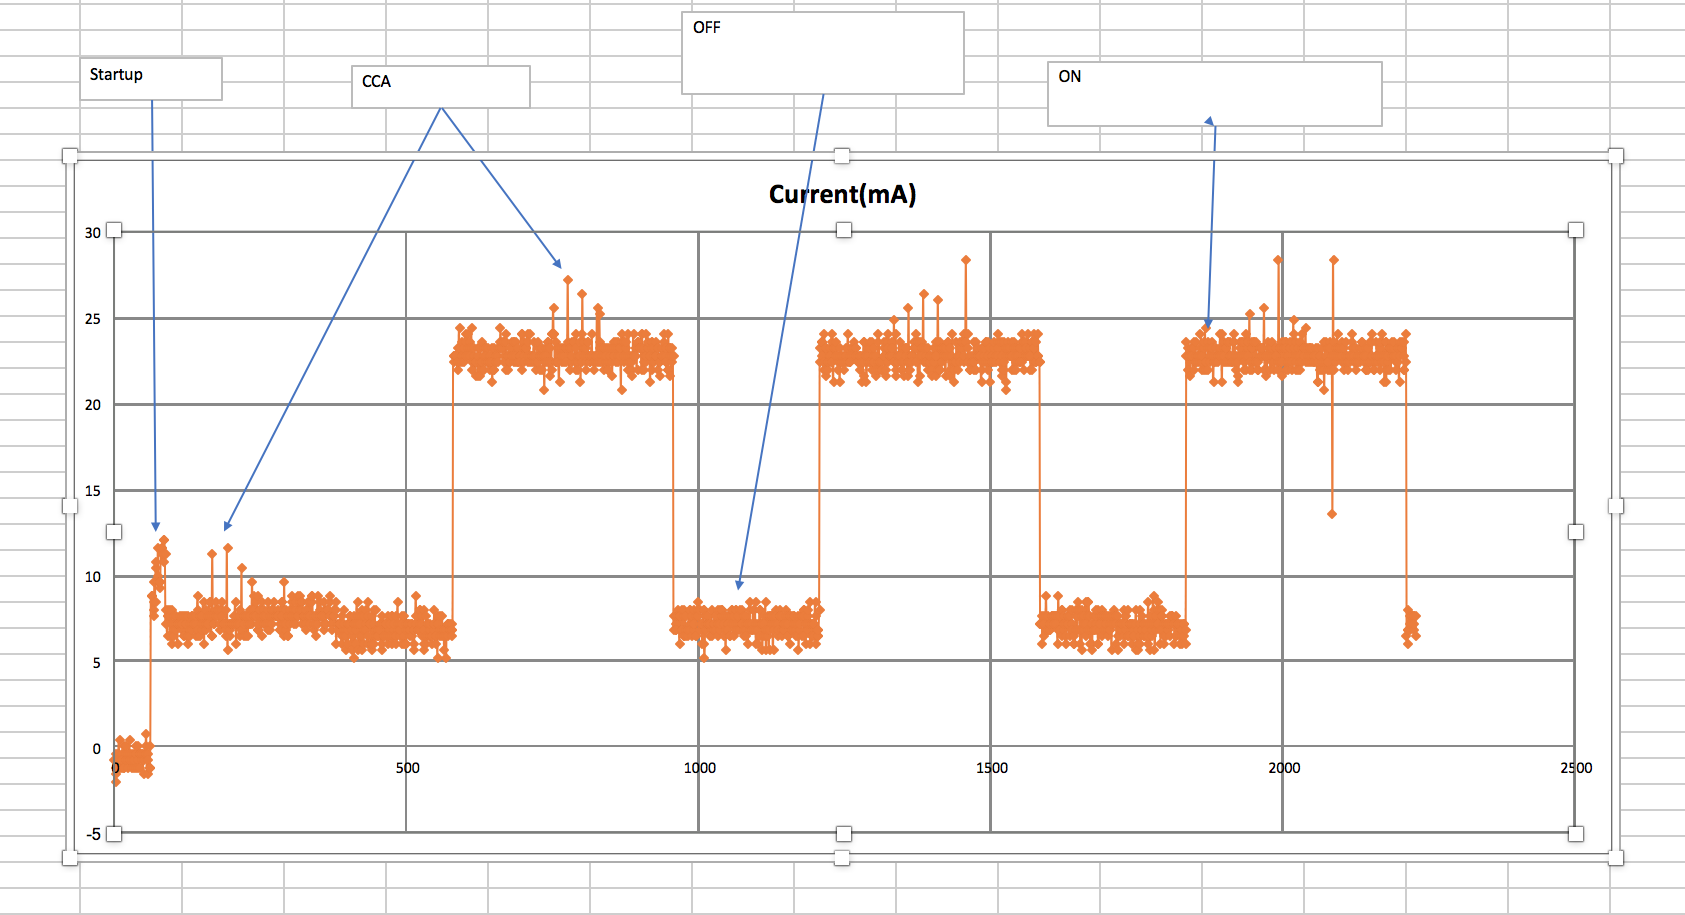
\includegraphics[scale=0.5]{power_profile}

\end{document}